%!TEX root = ../thesis.tex
\chapter{Results}
\label{ch:results}

In this chapter we present the results we compiled during the course of our work.
This includes an evaluation of the developed hexapod model and its locomotion controller, as well as review of the RL training results obtained and lessons learned from observing the training process.

\section{Evaluation: Hexapod model}
During the development process of the hexapod model and locomotion controller, we observed that the conceived model architecture enables us to quickly modify and/or add components.
An example of this flexibility is provided by the retrospective addition of sensor readings for the rotational acceleration of the \textalpha-joints.
As the hexapod leg is defined as a library component, it was only necessary to enable the respective sensor reading one the joint block and add the new signal to the already existing sensory information bus. 
There was no need to modify the hexapods legs individually, as Simulink automatically updates all library-linked blocks.
In general, the library of custom subsystems has proven to be a most useful tool, reducing development time and promoting modularity.
The encapsulation of the hexapod model as a whole into a single, top-level subsystem block that only reveals necessary in- and outputs, provides the developer with a simple to understand interface.
It also gives us the ability to duplicate the complete hexapod system without any effort, which could prove useful in future research as it enables the system to easily be utilized in multi-agent simulations.

Concerning the actual simulation of the model, it can be said that in most cases in which the robot uses a statically defined gait pattern for locomotion, a simulation step size of 0.5 ms yields stable results and runs at close to real time.
Given an untrained, exploring RL agent as the models operator, a step size of 0.25 ms is preferable, as sudden twitching and jerking motions might occur, which can lead to simulation instabilities and exceptions.
Similar to the results of \cite{thilderkvist2015motion}, we begin to observe these problems at larger step sizes ($> 0.5 ms$), although not of the same significance and frequency as described by them. 
The most common reason for exceptions we observed, were collision detection failures.
These occur, when two rigid bodies move into each other faster than the simulation's solver can observe, due to its limited temporal resolution.
During the several ten-thousand simulation episodes performed at a step-size of 0.25 ms during RL training, we did not once observe an exception.
Overall, the behaviour of our robot model seems, to the best of our knowledge, but without the co-examination of a real world counterpart, physically accurate.


We attribute the unsatisfactory results \cite{thilderkvist2015motion} experienced from the spatial friction forces to be most likely linked to deciding on a step size too large for stable simulations.
As they also work with an earlier MATLAB version, using Simscape's predecessor \textit{SimMechanics}, the problems might also have arisen from a possibly more primitive physics model.

To summarize, we were able to create a well-functioning, virtual model of a hexapod robot.
Simulations of the model are robust, physically accurate and performant.
We are confident that the model can serve as a platform for future research, as it utilizes a modular architecture, can easily be expanded and is based on the versatile MATLAB environment.
 

\section{Evaluation: Locomotion Controller}
The locomotion controller we presented in \ref{subsec: Locomotion controller} is the result of several design iterations.
We extensively tested each of the designs to uncover their weakpoints, upon which the next iteration was improved on.

To begin with, the initial design (\textit{MK1}) enabled the robot to walk in a straight line tripod gait.
We observed that the hexapod model, controlled by MK1, would jerk up and down significantly during a movement cycle, as can be seen in \hyperref[vid: MK1]{MK1} and \ref{figure: Thorax Height graph, bad tuning}.
During a legs swing phase, the robots thorax would slowly sink towards the side of the lifted leg and be rapidly pushed upwards again at the end of the swing.
As we defined the leg trajectory relative the thorax and did not consider sensing ground contact or body tilt, the leg on the sinking side would hit the ground earlier than expected by the controller, as the anticipated AEP "sunk" into the ground plane.
We were able to later on attribute this behaviour to the slow reactions of the PID controllers.
These were, given our initial tuning parameters ($K_p = 3, K_i = 0.2, K_d = 1, N = 100$), unable to follow their assigned trajectories. 
In addition, the MK1 controller version requires a lot of calculation time per simulation step, resulting in slow simulations.
The observed cause of this being the computationally intensive, iterative IK block provided by Simulink, as we have already elaborated on in \ref{subsubsec: IK Solver}.

With the subsequent version, \textit{MK2}, we focused on introducing tetrapod and wave gait as well as increasing simulation speed.
Implementing the gait patters proved to be straightforward, as, resulting from the models modular architecture, solely the leg coordination of the static gait definition had to be modified.
The resulting simulations of the robot walking in tetrapod and wave gait can be observed in \hyperref[vid: MK1]{MK2}.

The decision to implement our own, custom analytical IK solver resulted in a significant performance boost.
Comparing the MK1 and MK2 controllers, we are able to achieve an up to 5x speed up in simulation time.
Running a 30 second simulation of a hexapod walking in tripod gait, controlled by MK1, required a full x seconds of real compute time, while the same simulation takes about y seconds to run when the hexapod is controlled by MK2.

\todo{Prove with a comparison of MK1 and MK2 simulation time, run MK1 and MK2 on desktop}

With the final non-RL controller design, termed \textit{MK3}, we improved the stability of the hexapods locomotion as well as introduced the capability for omnidirectional movement.
By simply re-tuning the PID controller parameters to the values displayed in \ref{table: PID parameters}, we were able to reduce the jerking behaviour of the robot far enough to almost being visually unnoticeable.
A comparison of the thorax's height differences during movement, when under control of the MK2 and MK3 controllers, can be seen in Fig. \ref{figure: Thorax height graphs}.


\begin{figure}[h]
	\begin{subfigure}{\textwidth} % this sets the figure to be max half the width of the page
		\centering
		% include first image
		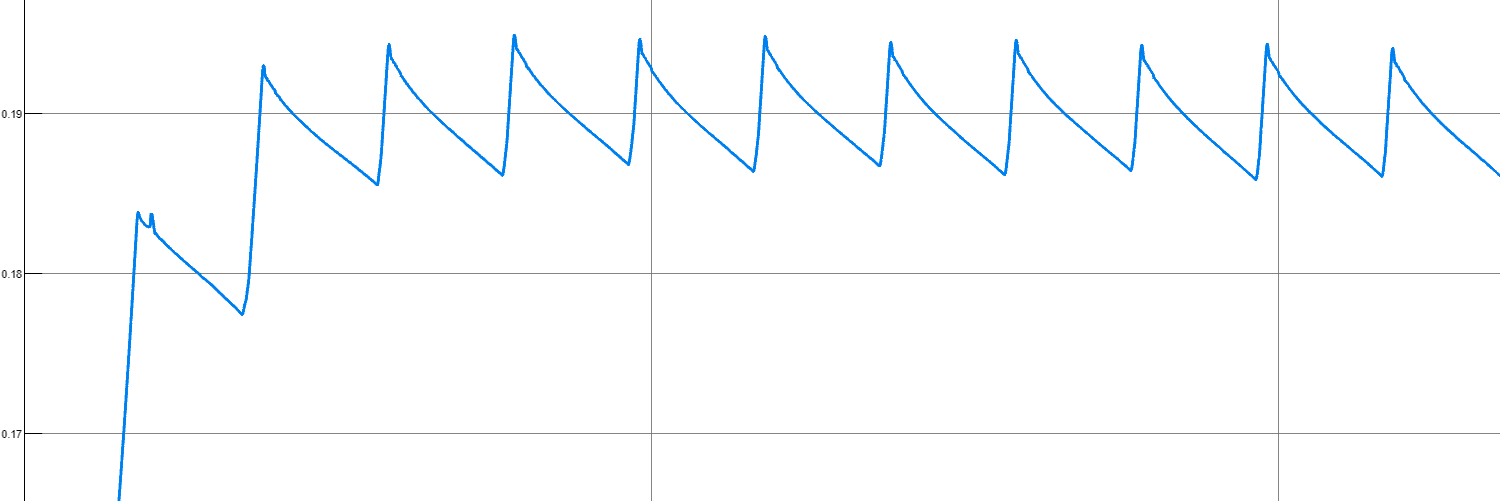
\includegraphics[width=\linewidth]{ThoraxHeight_firstPID.PNG}  % this sets the image to fill 90% of the available space -> 45% of the line width in total. 
		\caption{}
		\label{figure: Thorax Height graph, bad tuning}
	\end{subfigure}
	
	\begin{subfigure}{\textwidth}
		\centering
		% include third image
		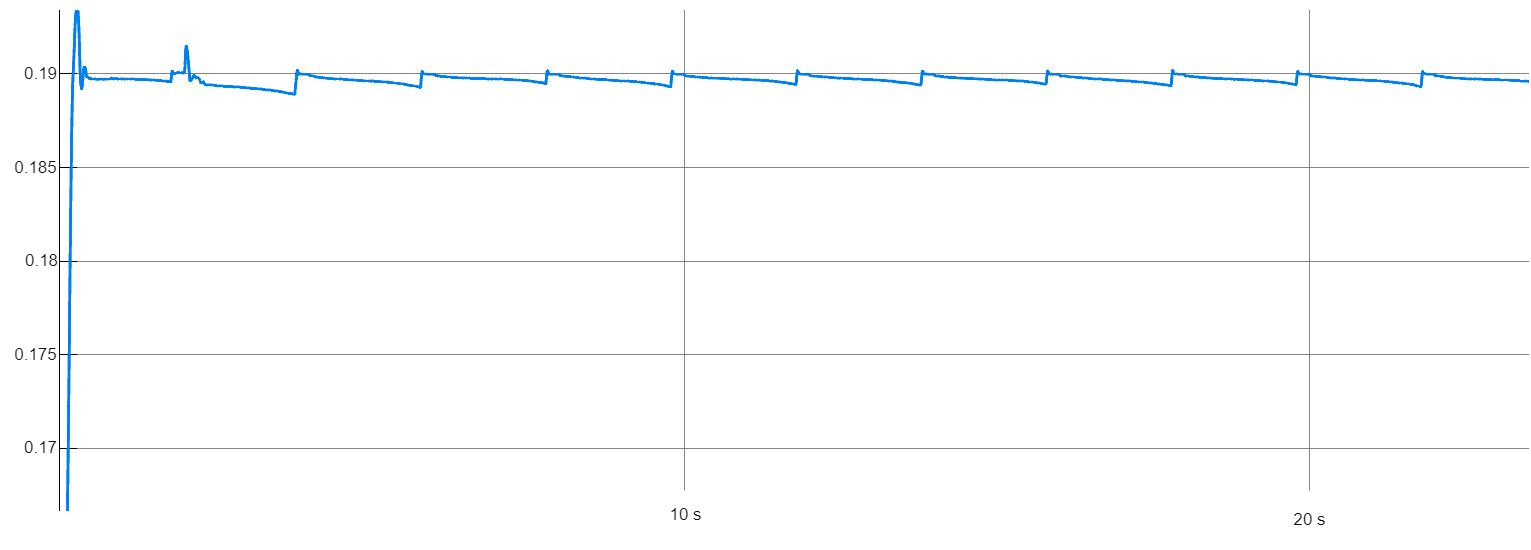
\includegraphics[width=\linewidth]{ThoraxHeight_retunedPID.PNG}   % this width should be half of the width of the other two images
		\caption{}
		\label{figure: Thorax height graph, re-tuning}
	\end{subfigure}
	\caption[Thorax height graphs]{(a) Thorax height graphs of hexapod robot controlled by (a) MK2 and (b) MK3 controller.}
	\label{figure: Thorax height graphs}
\end{figure}

Our final, MK3 locomotion controller is able to control the hexapod model in tripod, tetrapod as well as wave gait.
The swing-stance cycle frequency ($f_c$) and the duty cycle percentage ($P_\text{swing}$) can be changed, even dynamically during simulation.
We demonstrate this dynamic frequency alteration with a hexapod model walking in wave gait with varying cycle frequency.
The controller initiates movement with a $f_c$ of 0.1 Hz, slowly increasing over 20 seconds linearly to 0.5 Hz. 
It is also possible to redefine the step height and AEP/ PEP positions.
As already mentioned, the final controller is capable of instructing omnidirectional movement, as we demonstrate in a study of the robot walking in a circle.
Additional studies of the hexapod robot performing all predefined gait patterns at different cycle frequencies were performed.
We captured all of the simulations mentioned above a videos wich can be viewed at (\hyperref[vid: MK1]{MK3}).

Concerning the hexapods ability to navigate obstacles or uneven terrain, it has to be noted that the controller does not possess any means of observing environmental details, thus not being able to distinguish between terrains.
It therefore struggles to overcome small obstacles put in its path.
We explored the robots performance at overcoming a 10 cm wide an 4 cm high beam, perpendicular to the robots movement direction.
Summarizing the findings of simulations in all available gaits, the hexapod walking in tripod gait was able to eventually overcome the obstacle, while it struggled to do so in both tetrapod and wave gait, given the allotted timespan of 60 s.
We attribute the tripod gait's success to the fact that it presents the lowest number of legs in stance at any point in time, as we observed that legs in stance often get caught on the obstacle.
Due to the nature of our controller, legs in their stance phase are rather reluctant to deviation from their trajectories, thus when caught in from of the obstacle, preventing the robot from moving forward.
Videos of the obstacle simulations can be observed in \hyperref[vid: MK1]{MK3}.


\section{Evaluation: RL training}

Implementing a RL agent yielding satisfying results proved to be more difficult than anticipated.
As there exists a large set of parameter to be considered during setup, finding a well-performing set has shown to be a time-consuming task.
This was reinforced by the fact that, to observe the performance of a set of parameters, we found the agents to require at least 1-2k episodes of training, equating to several hours of runtime given the hardware used.
Additionally, as we ran experiments with two different RL algorithms, we were required to tune two separate sets of parameters.
In total, we trained over 30 agent configurations, each with a different set of parameters.
As we are not able to present all the results obtained, we focus only a selected subset.
Although a table providing information about all documented configurations is provided in the appendix (\emph{\nolinkurl{RL_agent_configs.xlsx}	}).

We were unsuccessful in our task to train an agent which can perform a stable gait pattern.


\subsection{Reward Exploitation}
A general problem often observed in RL is an agent exploiting a poorly-defined reward function \parencite{silver2015}.
This commonly leads to agents exhibiting undesirable behaviour, even though according to the reward function they are performing well.
We experienced this exploitation behaviour during our experiments as well.
As our reward function initially did not take into account the robots energy consumption nor height differences of the thorax during movement, early RL agents exploited this simpler reward function by learning to jump.
More specifically, we observed the robot exhibiting	 a behaviour consisting of small, abrupt hops, using it's hind legs to propel itself forward.
We provide a recording of the observed behaviour in \hyperref[vid: MK4]{MK4}, the training graph of the agent can be seen in \ref{}.
In this graph, the occurrence of the exploit is clearly visible as a spike in the average reward that quickly breaks down again.

\subsection{Learning Behaviour}
The phenomenon of sharp spikes in the average reward mentioned above, persisted throughout our training runs, occurring on several different agent configurations.
Another training graph depicting ths behaviour can be seen in Fig. \ref{}.
We suspect these reward plunges to be related to the agent exploring to rapidly/ changing it's policy to fast, resulting in it loosing the progress already achieved \parencite{silver2015}.
However, were cannot prove this cause as we are not able to reliably prevent the behaviour.

On the other hand, in stark contrast to the phenomenon just explained, we also observed "flatlining" of the average reward.
An agent would often learn well initially, but after a certain number of episodes converge to an average reward well below the reward unique episodes obtained.
Interestingly, this behaviour could very well be attributed to the agent's exploration not being aggressive enough, such that it is unable to leave a locally optimal policy \parencite{silver2015}.
Despite our efforts to find a middle ground between these two extremes by changing the agent's learning rate an introducing varying amounts of randomness into it's decision process, we were not able to find a well-working configuration.

Given the weights of the reward function in table \ref{table: Reward weights}, a sample rate of 0.05 s and an episode length of 256 steps, a statically defined tripod gait is able to obtain a reward of $\sim785$ units, while the best RL agent we were able to train achieved a maximum episodic reward of <310 units.
This equates to the RL agent performing 40\% as well as the fastest statically defined gait.
In this training run, performed with a DDPG agent which parameters are displayed in \ref{table: DDPG parameters}, the average reward did neither spike nor converge to a suboptimal policy, as can be seen in \ref{}.
Even though, the average reward does not seen to reliably increase.
A demonstration of the best performing policy obtained from this training run can be seen in \hyperref[vid: MK4]{MK4}.

When we first started working on the RL process, te result were not very promising. The agent did stabilize, meaning it did not jump around randomly, but it was not able to find an efficient gain.
The agent never learned to reliably move a leg forward if it was starting to drag behind due to reaching the PEP.


As there were no significant differences in performance to be observed between the DDPG and PPO algorithms, we abstain from comparing them separately.
As the learning ability of both algorithms was observed to be about equal, the RL algorithm can probably  be ruled out as a cause for the unsatisfactory results. 


As we changed the reward function several times in attempts to improve it's performance evaluation, the training episodes cannot be compared with the raw numbers.
Instead, we focus on the development of the average and peak rewards over time, the convergence or divergence, etc.


The survival reward $r_\text{survival}$ is set at 0.1, resulting in the agent receiving $0.1 \cdot 512 = 51.2$ cumulative reward from survival during a full episode.


The graphs below each depict the learning curve of a RL agent. The dark blue graph represents the average reward (running average over the last 250 Episodes) and each data point on the light blue graph represents the reward of a specific episode.

{\def\arraystretch{1.4}\tabcolsep=5pt
	
\begin{table}
	\parbox{.4\linewidth}{
		\centering
		\begin{tabular}{| c | c |} 
		\hline
		\textbf{Training params.s} & \textbf{Value} \\ [0.5ex] 
		\hline
		\hline
		Sample time & 0.05 s \\ 
		
		Episode steps & 512 \\
		
		\hline
		\textbf{Agent params.} &  \\ [0.5ex] 
		\hline
		
		Learn Rate & $\num{3e-4}$ \\
		
		Episode steps & 512 \\
		
		Exp. Buf. length & $\num{1e6}$ \\
		
		Discount factor &  0.99 \\
		
		Mini-Batch size & 32 \\
		
		NN-width & 128 \\
		
		\hline
		\textbf{Noise params.} &  \\ [0.5ex] 
		\hline
		
		\textsigma\footnote{\textsigma: Standard Deviation} & 0.05 \\
		
		\textsigma-decay\footnote{\textsigma-decay: Decay rate of \textsigma. Each sample time step k, \textsigma decays according to following formula: $\sigma_{k+1} = \sigma_k \cdot (1 - \textbf{\textsigma-decay})$} & 1e-6 \\
		
		\hline
	\end{tabular}	
	\caption[DDPG agent parameters]{}
	\label{table:DDPG parameters}
	}
	
	%\hfill
	
	\parbox{.4\linewidth}{
		\centering
		\begin{tabular}{| c | c |} 
		\hline
		\textbf{Training params.} & \textbf{Value} \\ [0.5ex] 
		\hline
		\hline
		Sample time & 0.05 s \\ 
		
		Episode steps & 512 \\
		
		\hline
		\textbf{Agent params.} &  \\ [0.5ex] 
		\hline
		
		Learn Rate & $\num{3e-4}$ \\
		
		Episode steps & 512 \\
		
		Exp. Buf. length & $\num{1e6}$ \\
		
		Discount factor &  0.99 \\
		
		Mini-Batch size & 32 \\
		
		NN-width & 128 \\
		
		\hline
		\textbf{Noise params.} &  \\ [0.5ex] 
		\hline
		
		dev (\textsigma) & 0.05 \\
		
		devdec & 1e-6 \\
		
		\hline
		\end{tabular}
		\caption[PPO agent parameters]{}
		\label{table:PPO parameters}
	}
\end{table}
}

{\def\arraystretch{1.4}\tabcolsep=5pt
\begin{table}
	\centering
	\begin{tabular}{| c | c |}
		\hline
		\textbf{Weight} & \textbf{Value}\\
		\hline
		\hline
		$c_{s_x}$   		&  1	\\
		$c_{v_x}$   	    &  50	\\
	  	$c_{v_y}$  		    &  1	\\
	  	$\Delta_h$  		&  1	\\
	  	$c_W$ 				&  0.025\\
		\hline
	\end{tabular}
	\caption[Reward weights]{}
	\label{table: Reward weights}
\end{table}
}


%We used the \textbf{D}eep \textbf{D}eterministic \textbf{P}olicy \textbf{G}radient (DDPG) algorithm, an actor-critic, model-free, online, off-policy RL method.
%The actor network consists of a 12-wide observation input layer followed by 3 100 neuron wide fully-connected layer, in between each of them a ReLU-layer to introduce non-linearity.
%Concluding the actor network is an output layer consisting of 6 neurons, one for each action channel.
%The architecture of critic network is more complicated, as it has to take in more informations.
%At the start this network consists of two separate branches, one taking as inputs X and one Y.
%On both branches the input layers are followed by a fully-connected and a ReLU layer.
%At this point the two branches are connected by a simple addition layer.
%After the add-layer, another 2 combinations of fully-connected and ReLU layer follow, concluding with a single output neuron, representing the critics reward estimation.
%All of the actor and critic layers are, if not mentioned otherwise, 100 neurons wide.
%The architectures of the actor and critic networks have been adopted from example applications created by \cite{matlabDDPGExample, matlabPPOExample}.

%We used a learning rate of $3e^{-4}$ and $1e^{-3}$ for the actor and critic respectively and a discount factor of 0.99.
%The agents sample rate is set at 0.05, meaning the agent samples the environment and takes an action every 50 ms.
%A more detailed summary of the RL parameters is given in table \ref{table: DDPG parameters}.

{\def\arraystretch{1.4}\tabcolsep=5pt
\begin{table}
	\centering
	\begin{tabular}{| l | c |}
		\hline
		\textbf{Parameter} & \textbf{Value}\\
		\hline
		\hline
		Actor learn rate & $3e^{-4}$ \\
		Critic learn rate & $1e^{-3}$ \\
		Discount factor &  0.99 \\
		Mini-Batch-Size & 16 \\
		Experience buffer & $1e^6$\\
		\textsigma \ (UB) & 0.2 \\
		\textsigma-decay (UB) & $1e^{-6}$ \\
		
		\hline
	\end{tabular}
	\caption[DDPG parameters]{DDPG parameters. Uhlstein-Beck (UB) noise model is used to introduce noise into the agents exploration}
	\label{table: DDPG parameters}
\end{table}
}


\begin{figure}[h]
	\begin{subfigure}{\textwidth} % this sets the figure to be max half the width of the page
		\centering
		% include first image
		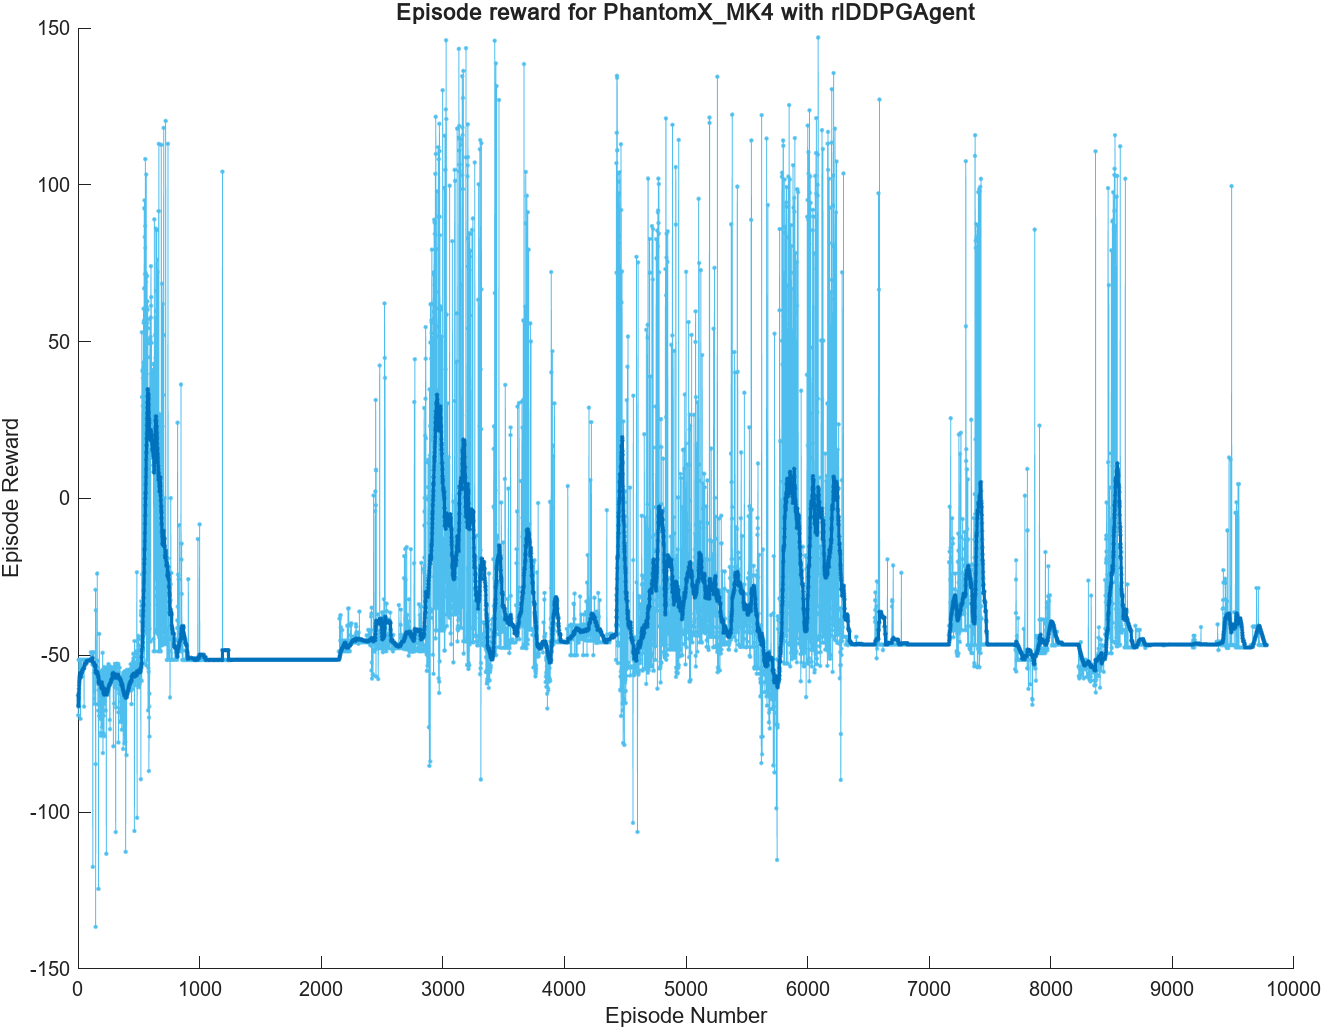
\includegraphics[width=\linewidth]{graphs/firstSuccess_146reward}  % this sets the image to fill 90% of the available space -> 45% of the line width in total. 
		\caption{}
		\label{figure: RL a}
	\end{subfigure}
	\begin{subfigure}{\textwidth}
		\centering
		% include second image
		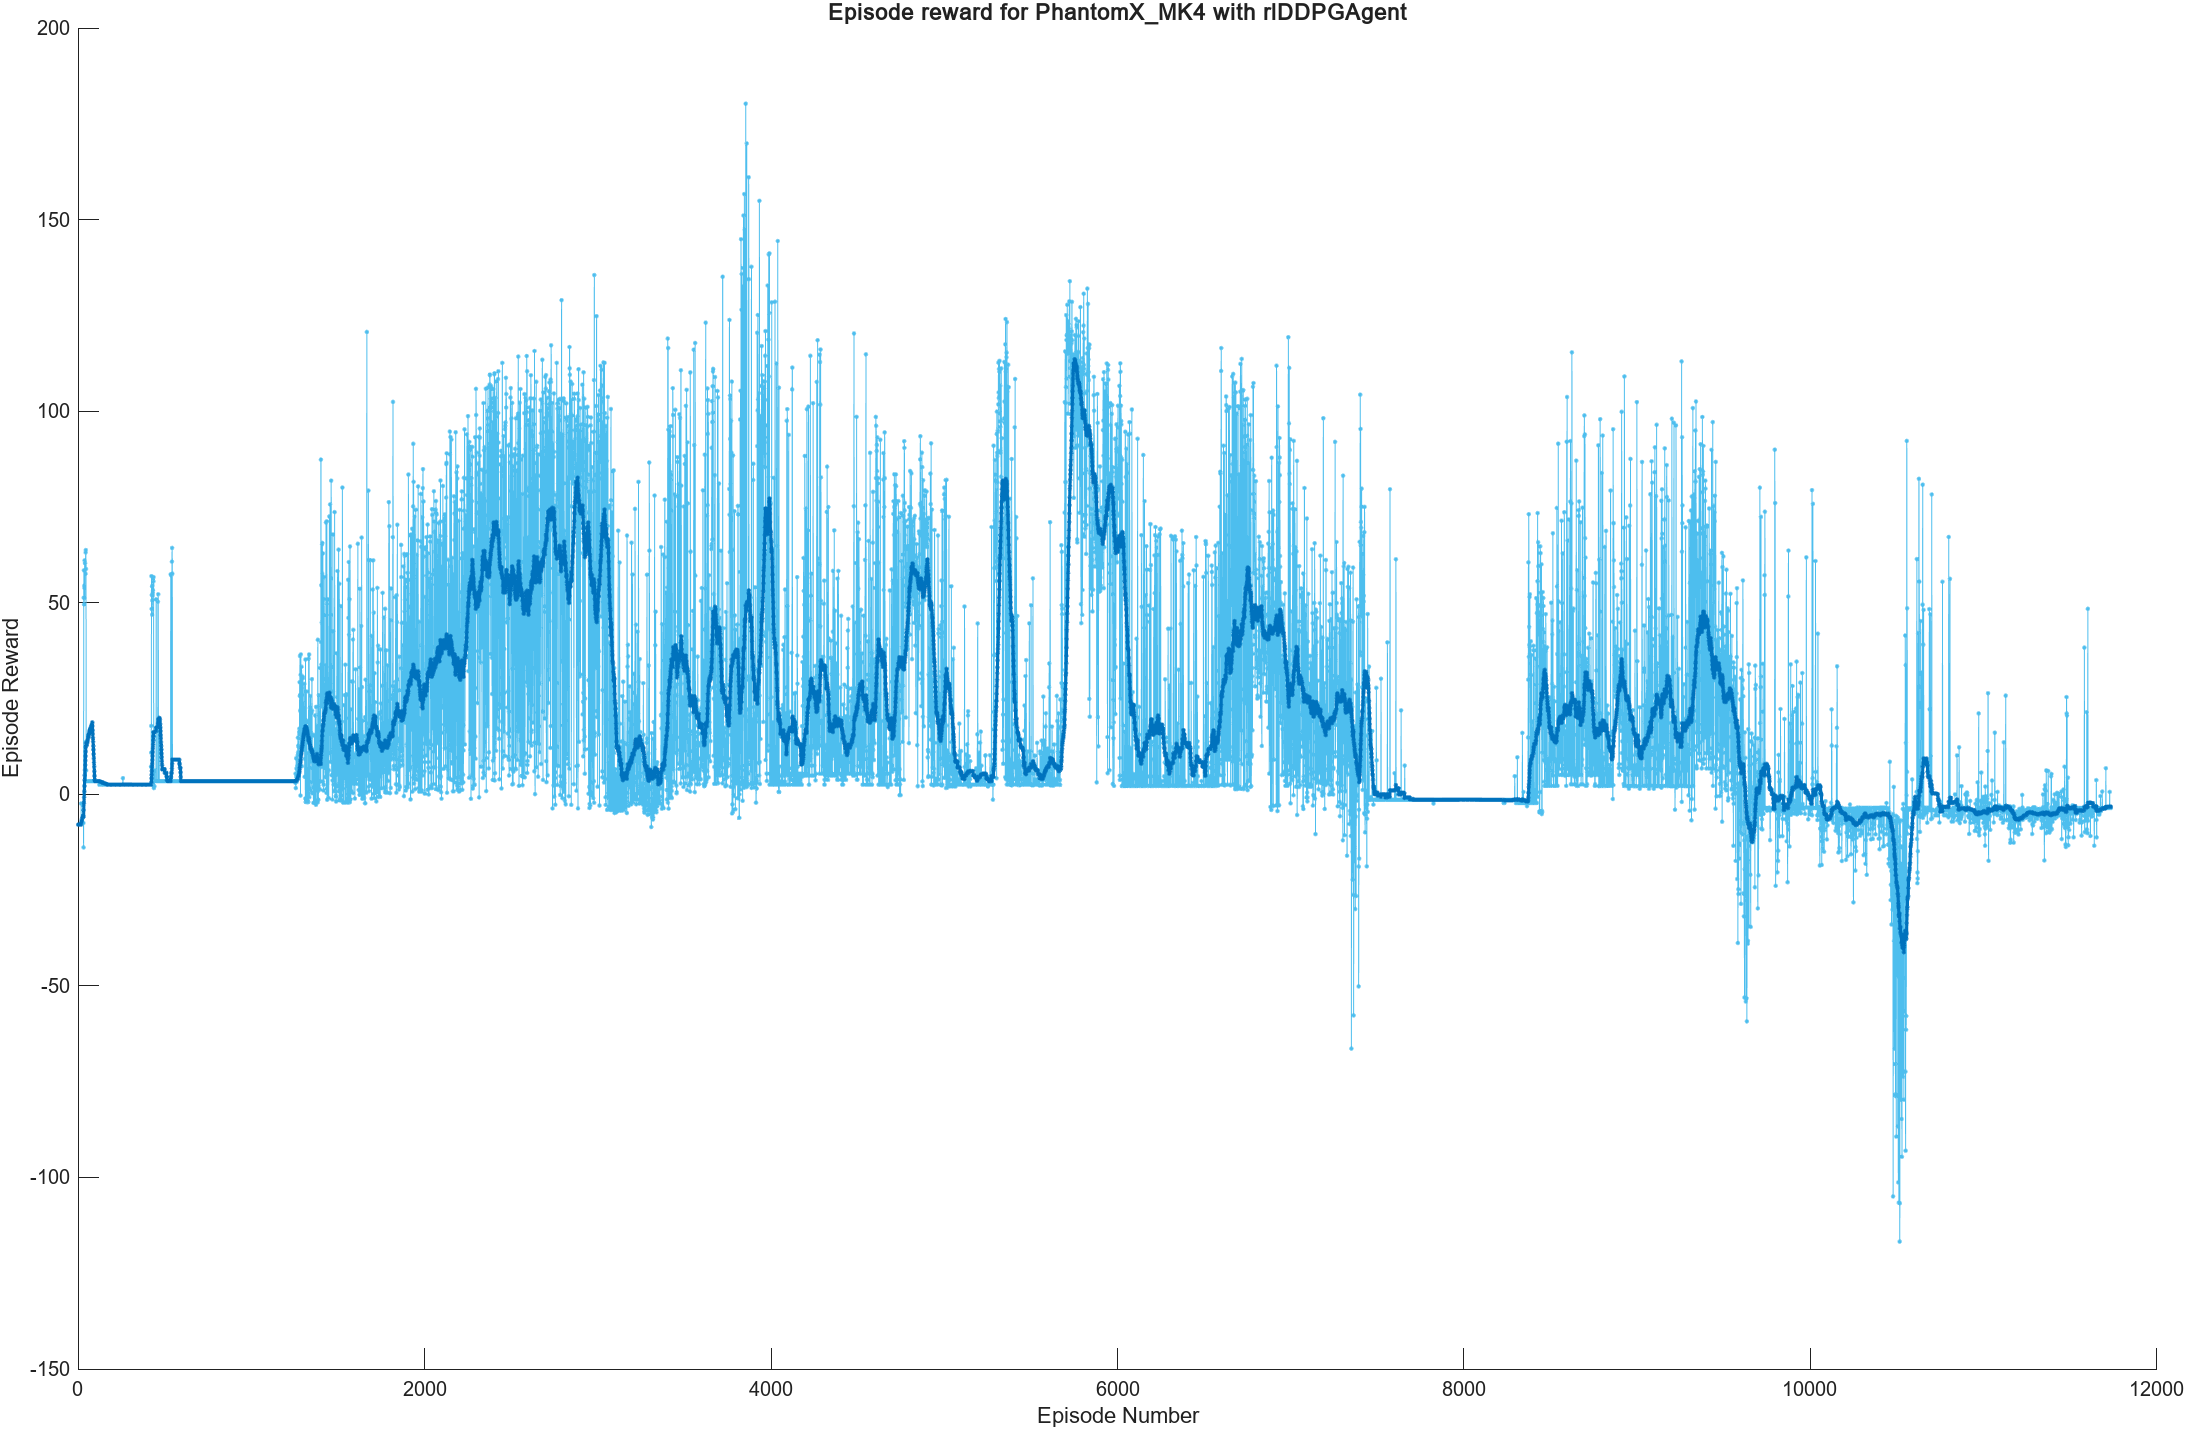
\includegraphics[width=\linewidth]{graphs/DDPG_reward_180.PNG}  
		\caption{}
		\label{figure: RL b}
	\end{subfigure} 
		\caption[DDPG training graphs (1)]{DDPG training graphs (1). (a) first Success 146. (b) DDPG Reward 180.}
	\label{figure: DDPG learning graphs 1}
\end{figure}

\begin{figure}[h]
	\begin{subfigure}{\textwidth} % this sets the figure to be max half the width of the page
		\centering
		% include first image
		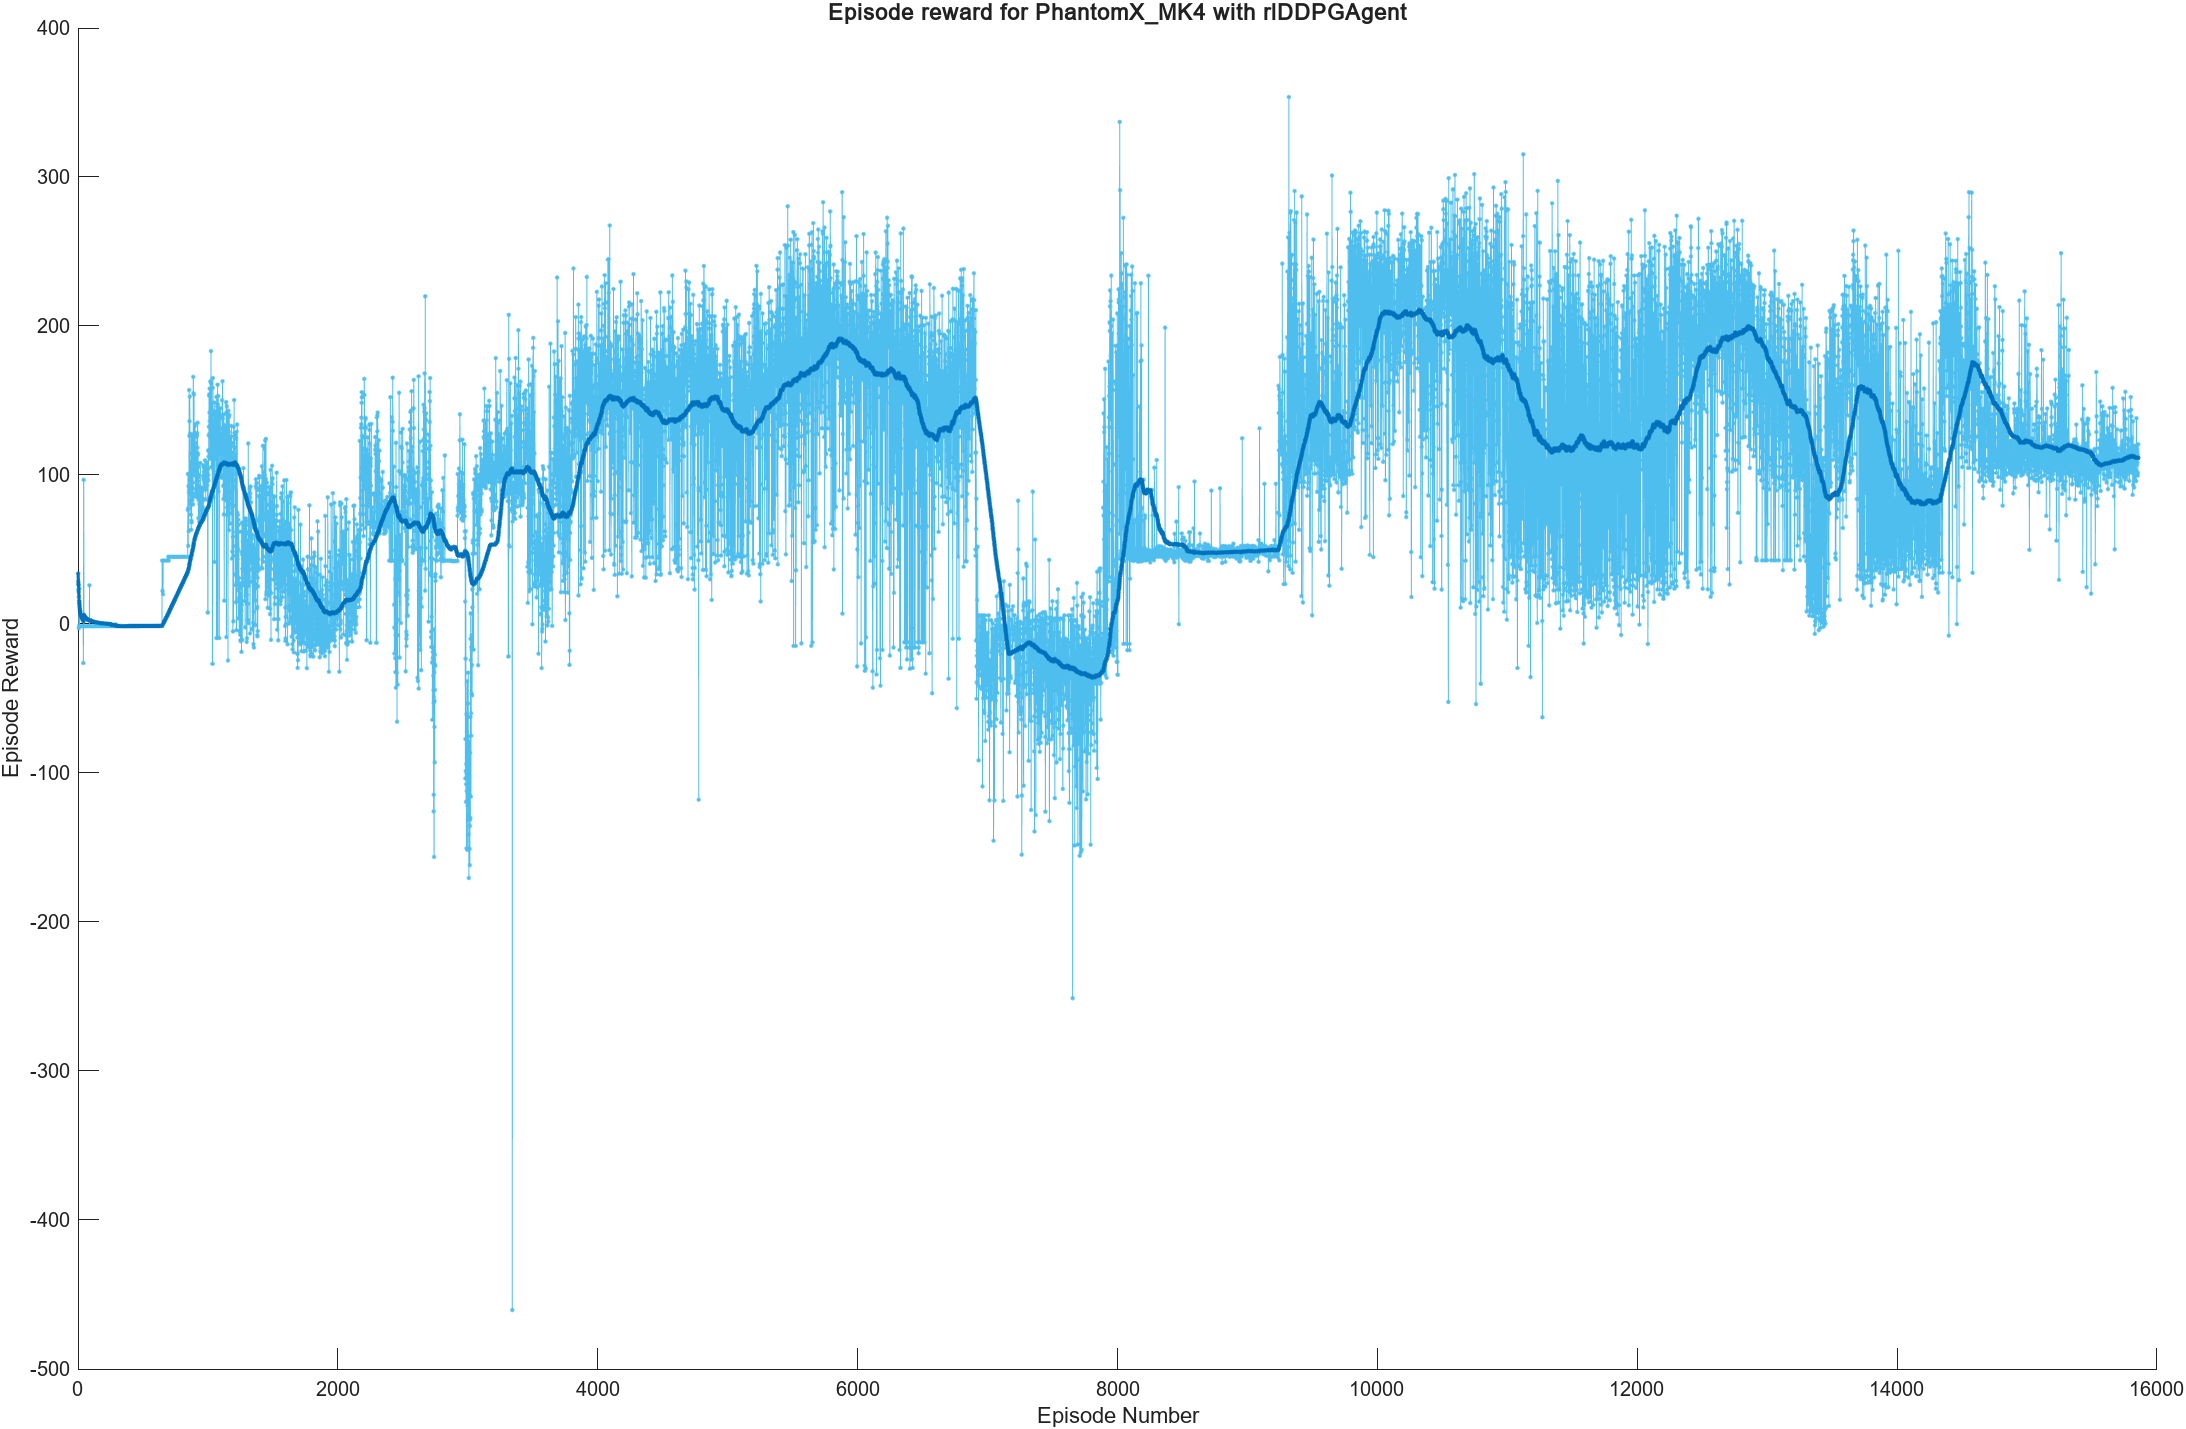
\includegraphics[width=\linewidth]{graphs/redefinedReward_50x_vx.PNG}  % this sets the image to fill 90% of the available space -> 45% of the line width in total. 
		\caption{}
		\label{figure: RL c}
	\end{subfigure}
	\begin{subfigure}{\textwidth}
		\centering
		% include second image
		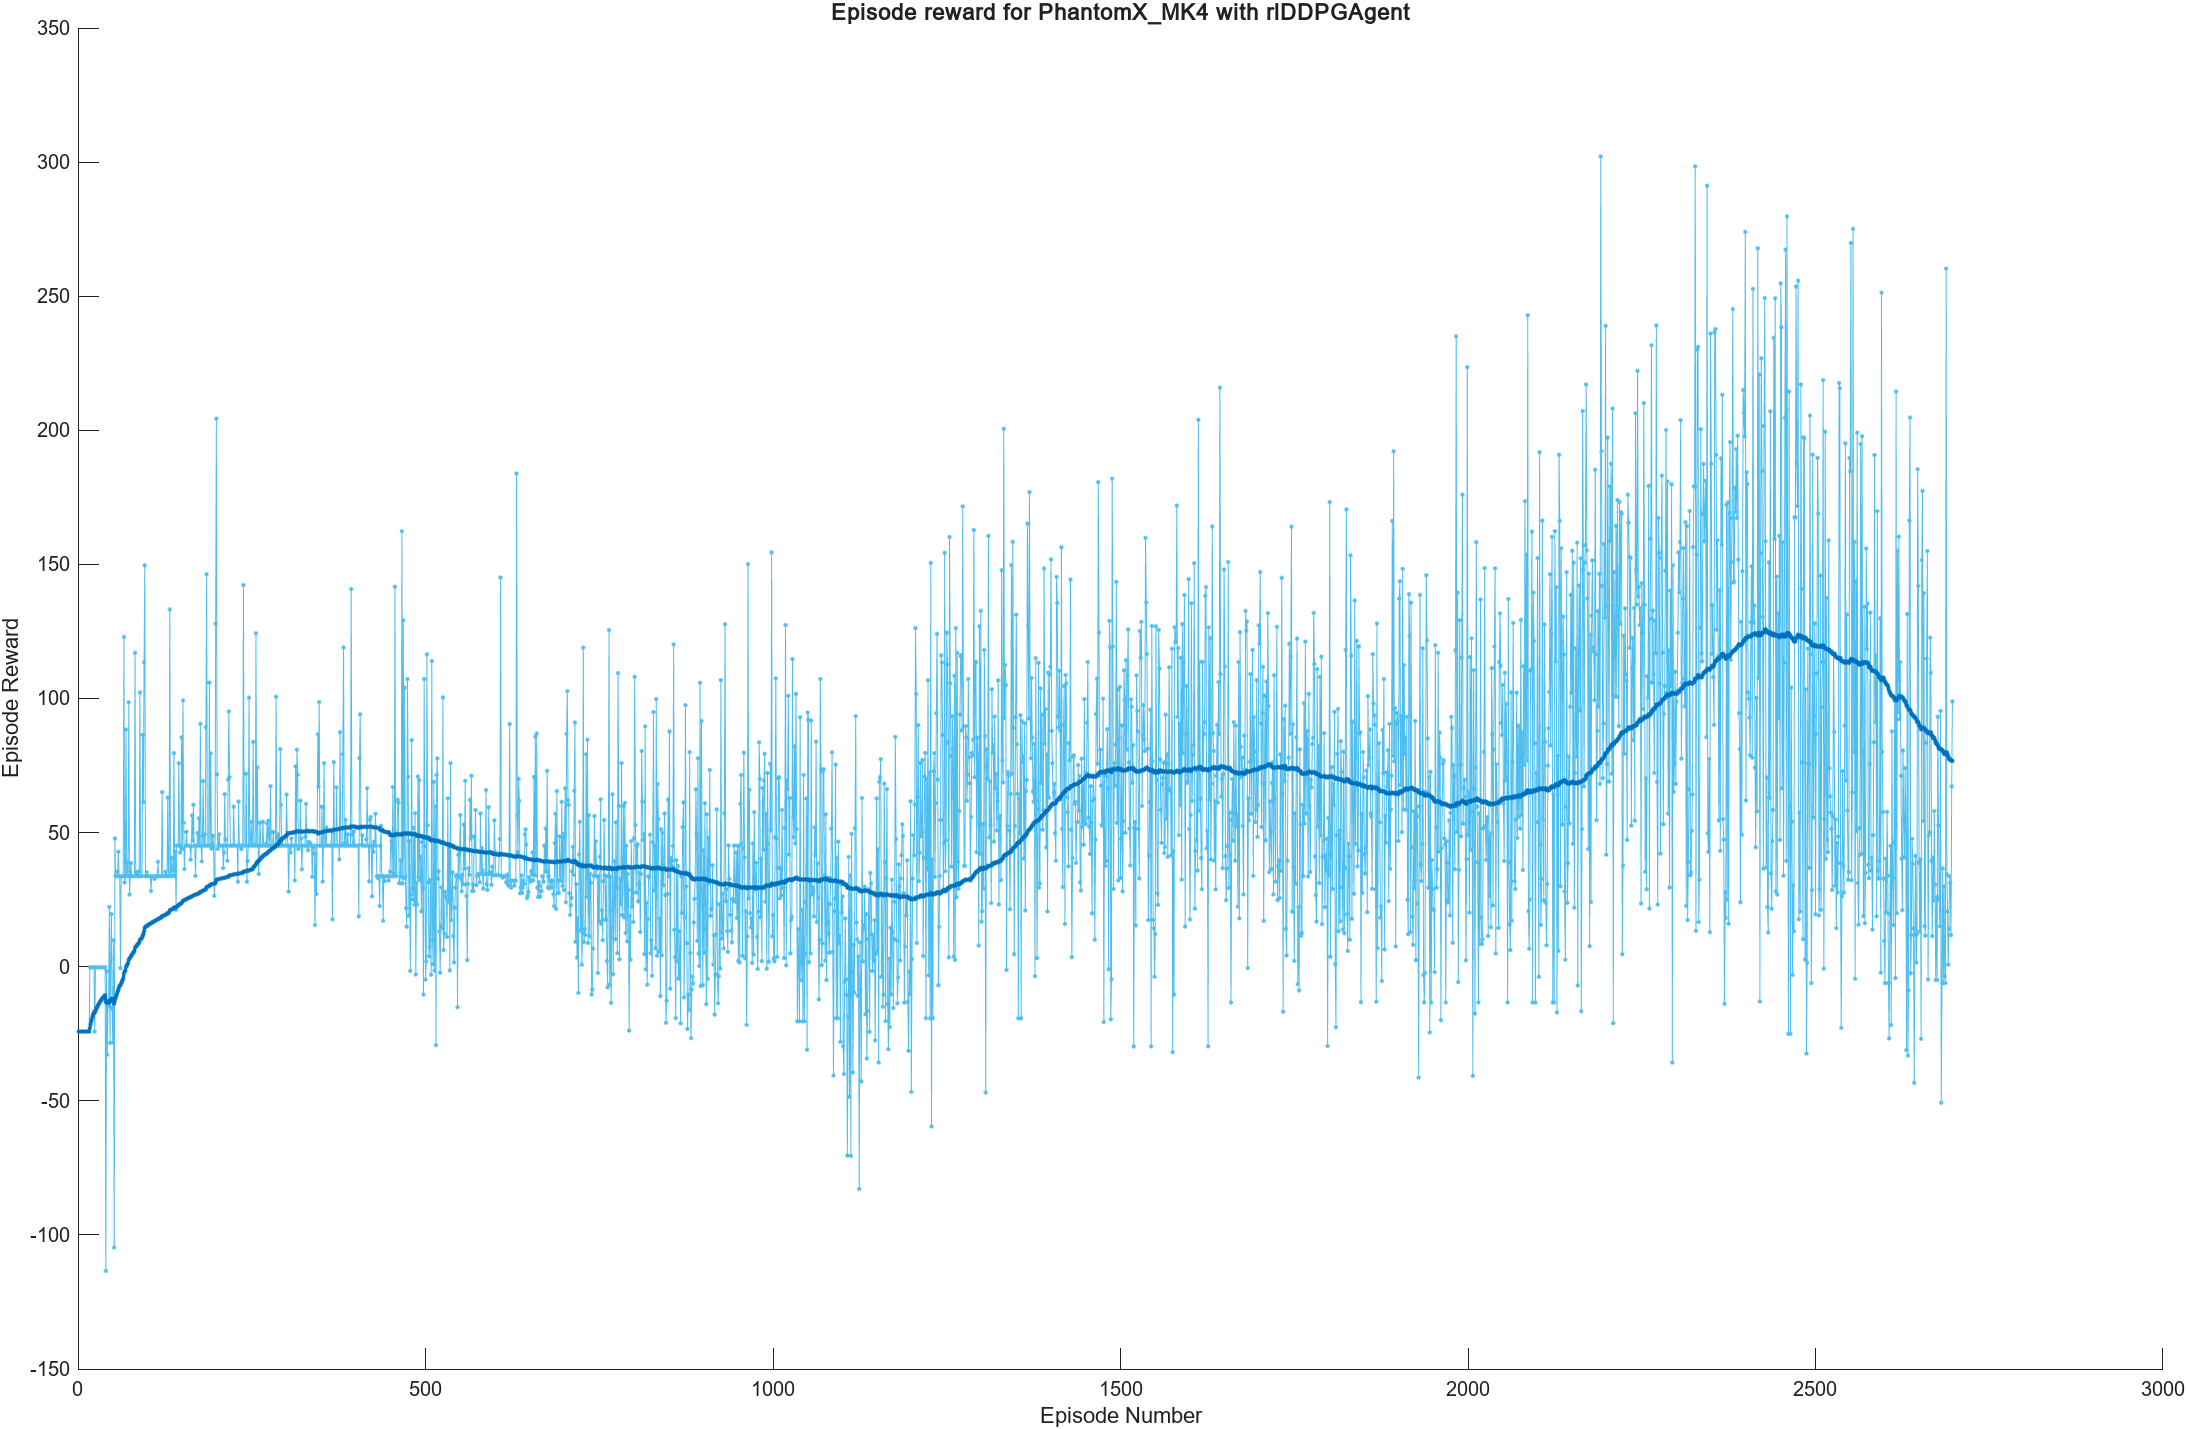
\includegraphics[width=\linewidth]{graphs/lastAgent_graph}  
		\caption{}
		\label{figure: RL d}
	\end{subfigure} 
	\caption[DDPG training graphs (2)]{DDPG training graphs (2).  (a) redefined Reward 50x vx. (b) lastAgent.}
	\label{figure: DDPG learning graphs 2}
\end{figure}


\subsection{Hardware}
The simulation studies and RL training performed for this thesis were all done on a desktop computer powered by an Intel i7-11700K CPU, 32 GB of RAM and a NVIDIA RTX 2060 GPU.
Concerning MATLAB, we used version 2023a for all of our work.

